\begin{figure}[tb]
    \centering
    \begin{subfigure}[tb]{0.48\textwidth}
        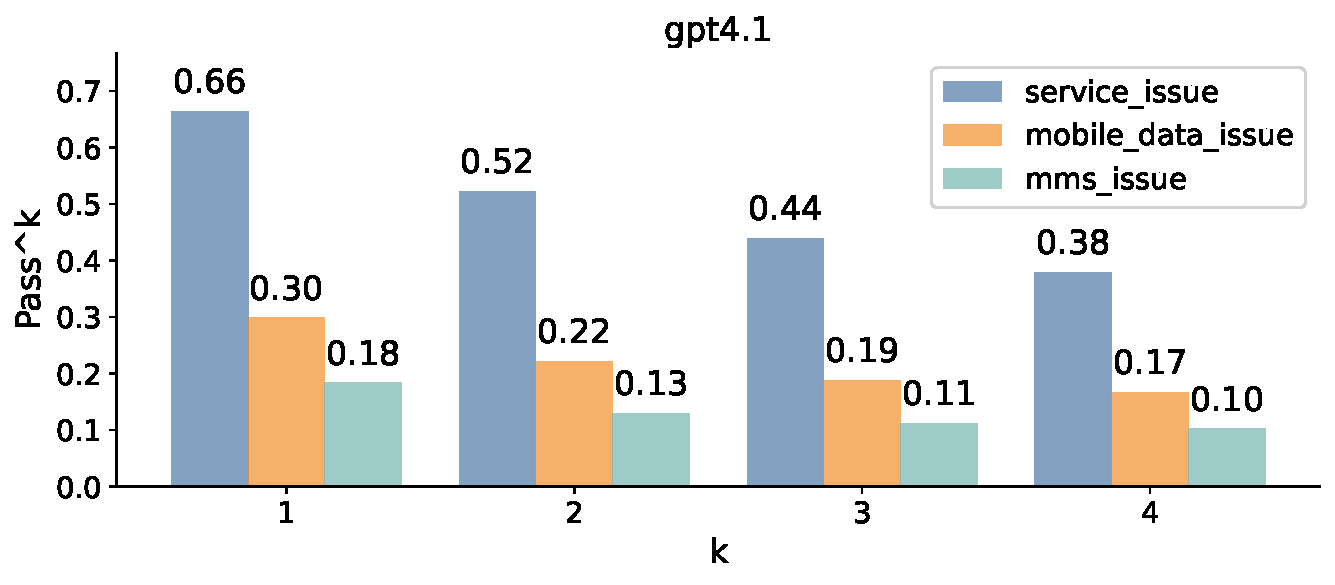
\includegraphics[width=\textwidth]{figures/results/pass_k_vs_k_per_intent_telecom_gpt-4.1-2025-04-14.pdf}
    \end{subfigure}
    \hfill
    \begin{subfigure}[tb]{0.48\textwidth}
        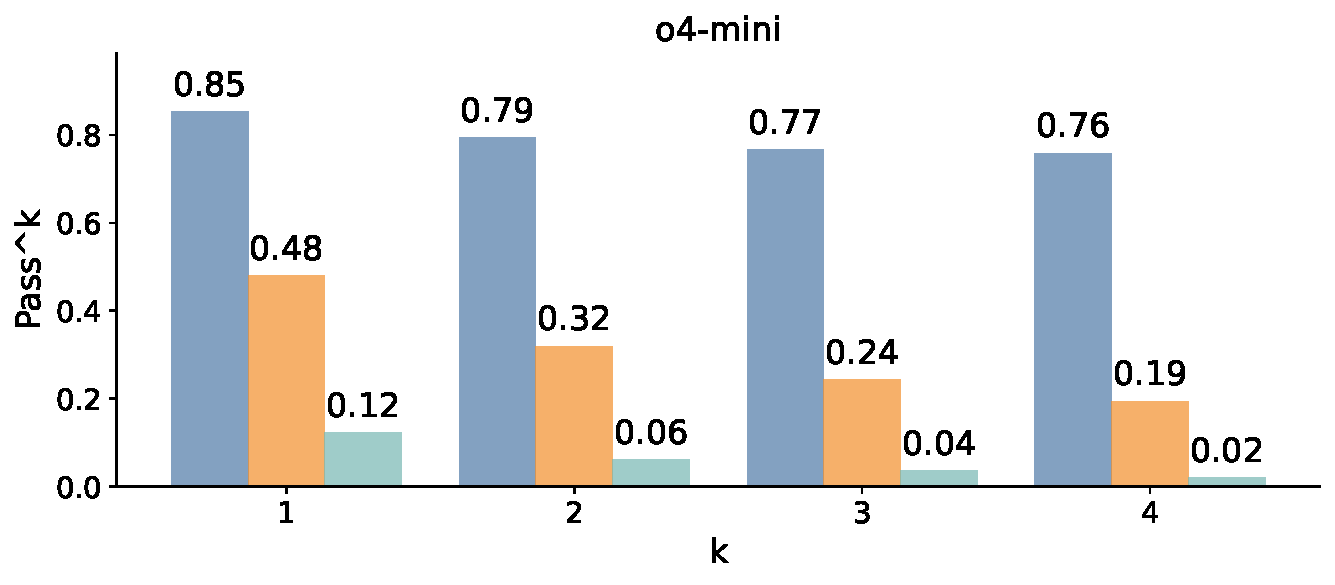
\includegraphics[width=\textwidth]{figures/results/pass_k_vs_k_per_intent_telecom_o4-mini-2025-04-16.pdf}
    \end{subfigure}
    \vspace{0.5em}
    \begin{subfigure}[tb]{0.48\textwidth}
        \centering
        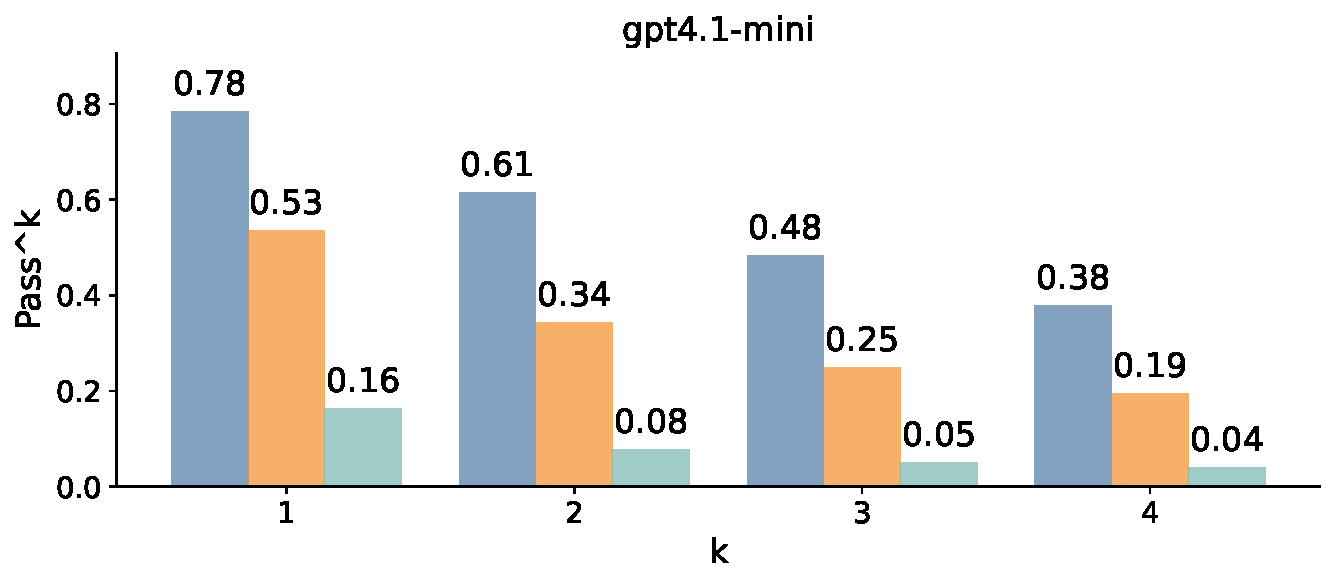
\includegraphics[width=\textwidth]{figures/results/pass_k_vs_k_per_intent_telecom_gpt-4.1-mini-2025-04-14.pdf}
    \end{subfigure}
    \hfill
    \begin{subfigure}[tb]{0.48\textwidth}
        \centering
        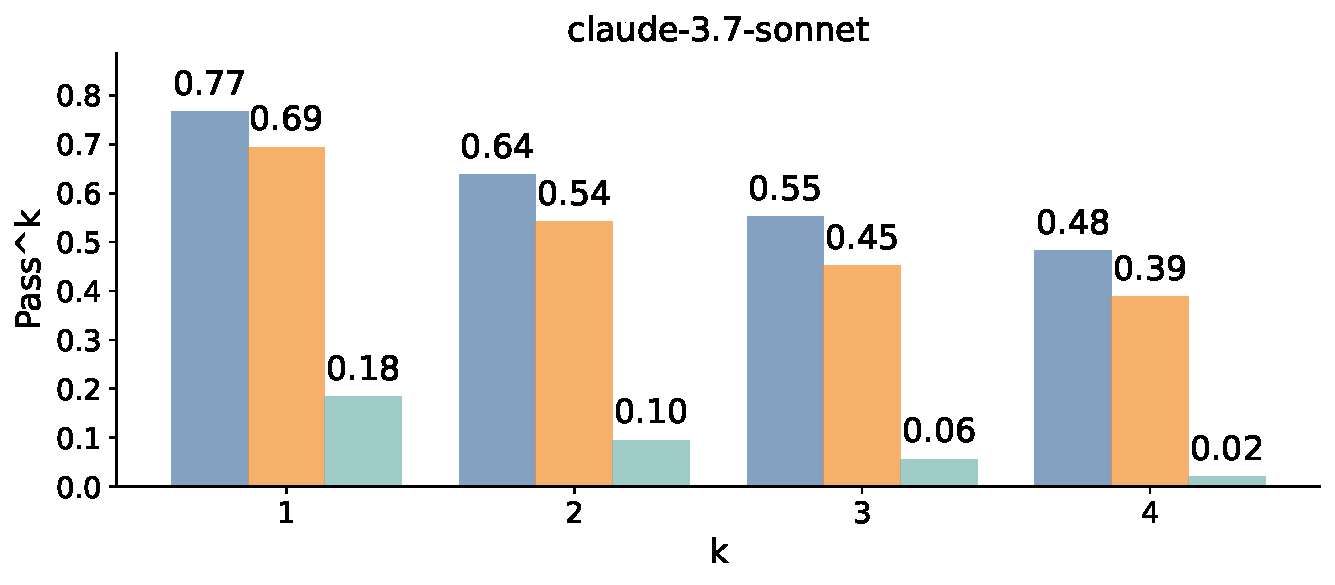
\includegraphics[width=\textwidth]{figures/results/pass_k_vs_k_per_intent_telecom_claude-3-7-sonnet-20250219.pdf}
    \end{subfigure}
    \vspace{-0.8em}
    \caption{\gptmodelshort (top left), \ofourmodelshort (top right), \gptminishort (bottom left), and \claudesonnetshort (bottom right) \passk per issue type for the \telecom domain. Performance is shown for \serviceissue, \mobiledataissue, and \mmsissue issue types, highlighting how different issue types affect success rates.}
    \label{fig:telecom_intent_results}
    \vspace{-1em}
\end{figure}

    
